\section{Summary of Findings} \label{section:summary_of_findings}

\subsection{Overview of the study objectives and what was undertaken}

This study investigated the extent to which machine-learned interatomic potentials (MLPs), specifically the MACE framework, can replicate interface favourability rankings computed via density functional theory (DFT) across various group-IV semiconductor systems, including carbon (C), silicon (Si), germanium (Ge), and tin (Sn). The project involved automated structure generation with ARTEMIS, interface relaxation via both DFT and MLP, and evaluation of rank preservation using statistical metrics including Spearman and Kendall correlations, as well as Top-N overlap.

\subsection{Recap of major results:}

\subsubsection{MLP vs DFT rank alignment}

The agreement between MLP and DFT was found to be system-dependent. MLPs performed well for Ge and Sn systems, achieving high rank correlation and overlap with DFT rankings. For Si, alignment was significantly poorer, with frequent rank reversals and diminished correlation metrics.

\begin{figure}[h]
    \centering
    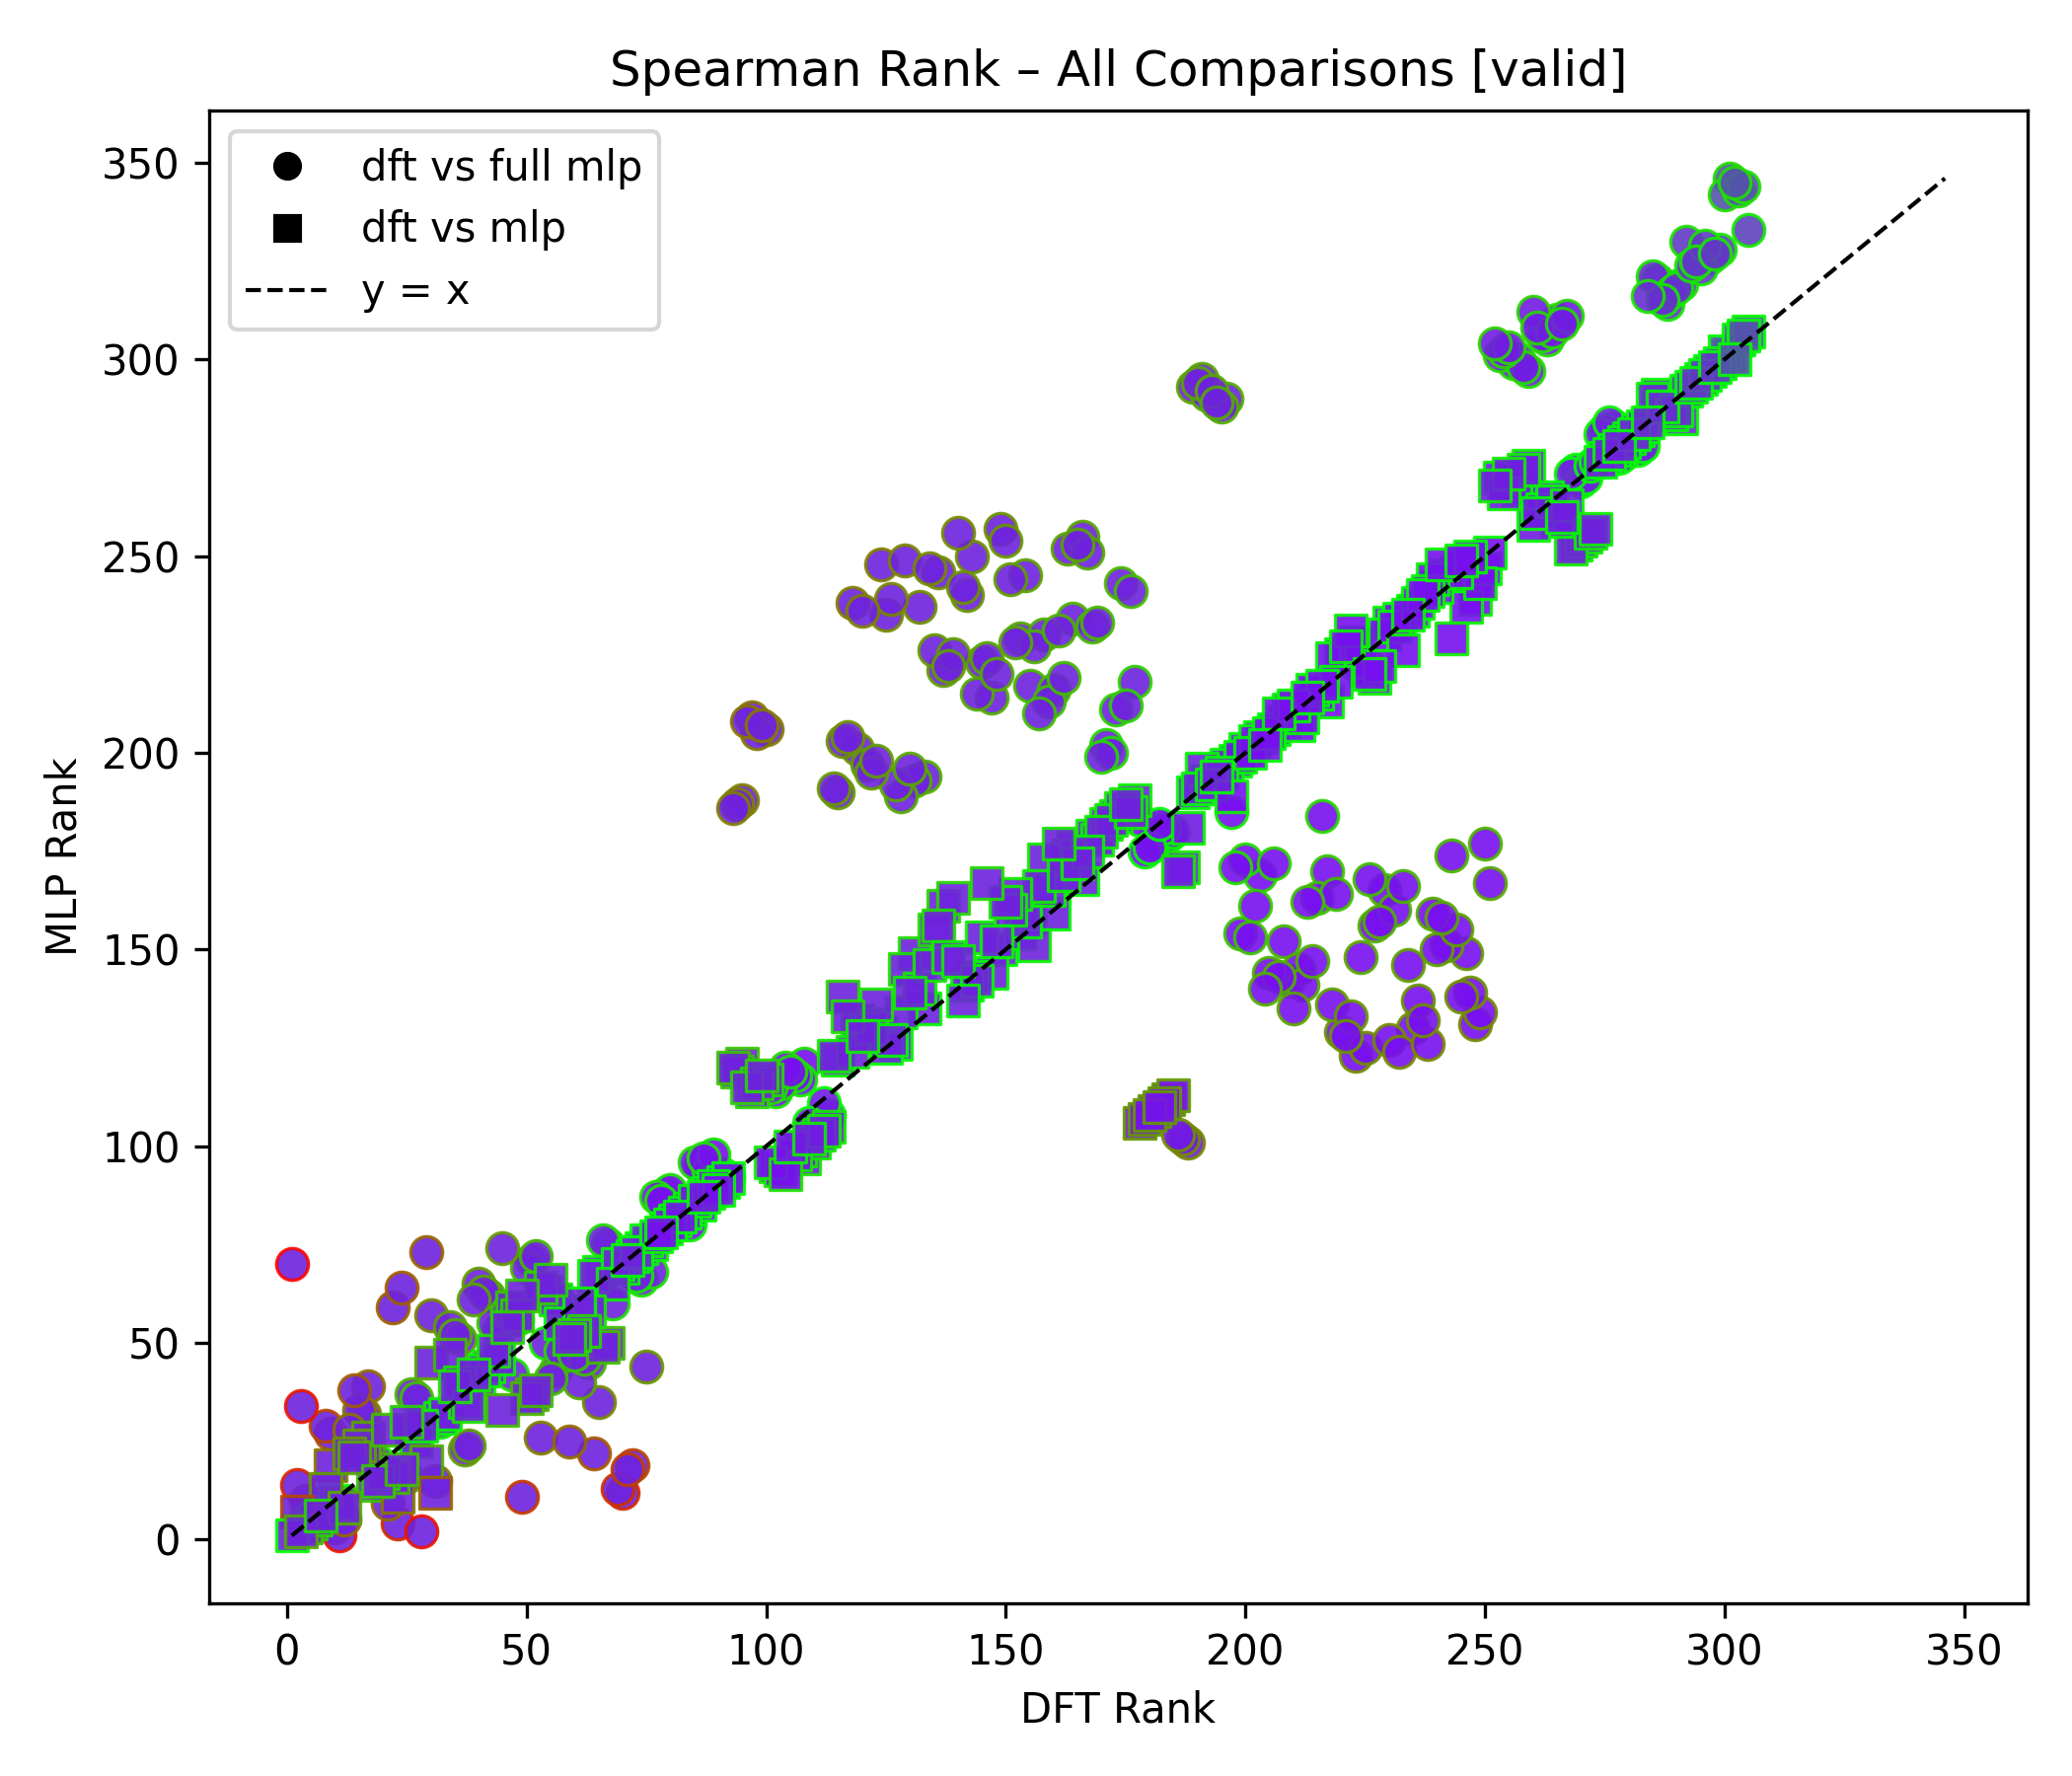
\includegraphics[width=0.7\textwidth]{analysis/plots/results_lower_Si_spearman_all_comparisons_valid.png}
    \caption{Spearman rank correlation for Si interfaces.}
\end{figure}

\subsubsection{System-specific performance (C, Si, Ge, Sn)}

Carbon results remain incomplete and thus inconclusive. Silicon systems exhibited persistent discrepancies between MLP and DFT rankings. Germanium and tin interfaces, by contrast, showed favourable agreement, with strong rank preservation and good Top-N screening utility.

\begin{table}[h]
    \centering
    \caption{Performance metrics for Si interfaces from \texttt{analysis/stats_upper_Si.csv}.}
    \begin{tabular}{lcccccc}
        Comparison & Spearman & Kendall & RMSE & MAE & Top-10 Overlap \\
        \hline
        DFT@DFT vs MLP@MLP & 0.46 & 0.31 & 7.48 & 3.36 & 3 \\
    \end{tabular}
\end{table}

\subsubsection{Value of cross-evaluation (e.g. DFT@MLP)}

Although direct MLP-on-DFT-relaxed structure evaluations (MLP@DFT) were not included due to computational cost, the study revealed that relaxation--evaluation consistency (e.g. MLP@MLP vs DFT@DFT) influences error, and future cross-evaluation may further clarify error sources.

% Placeholder for future figure showing relaxation-evaluation matrix comparisons.